\documentclass[11pt, a4paper]{article}
\usepackage[a4paper, margin=1in]{geometry}

\usepackage{adjustbox}
\usepackage{mathtools}
\usepackage{amsmath}
\usepackage{amssymb}
\usepackage{amsthm}

\usepackage{pgfplots}
\usepackage{listings}
\usepackage{color}
\usepackage{tikz}

\usepackage{textcomp}
\usepackage{soul}

\usepackage[hidelinks]{hyperref}
\pgfplotsset{width=7.5cm,compat=1.12}
\usepgfplotslibrary{fillbetween}
\pgfplotsset{compat=1.8}
\usepgfplotslibrary{statistics}
\usepackage[makeroom]{cancel}
\title{\bf{Homework \textnumero 18}}
\author{Author: David Oniani
\\
\ \ \ Instructor: Dr. Eric Westlund}
\date{April 21, 2019}

\usepackage{listings}
\usepackage{color}

%%%%%%%%%%%%%%% S E T S %%%%%%%%%%%%%%%
\newcommand{\nats}{\mathbb{N}}
\newcommand{\ints}{\mathbb{Z}}
\newcommand{\rats}{\mathbb{Q}}
\newcommand{\reals}{\mathbb{R}}
\newcommand{\irrats}{\mathbb{I}}

\newcommand{\pnats}{\mathbb{N}^+}
\newcommand{\pints}{\mathbb{Z}^+}
\newcommand{\prats}{\mathbb{Q}^+}
\newcommand{\preals}{\mathbb{R}^+}
\newcommand{\nreals}{\mathbb{R}^-}

\newcommand{\nints}{\mathbb{Z}^-}
\newcommand{\nrats}{\mathbb{Q}^-}
%%%%%%%%%%%%%%%%%%%%%%%%%%%%%%%%%%%%%%%

% Calligraphy
\newcommand\und[1]{\underline{\smash{#1}}}

% Operators
\DeclarePairedDelimiter\abs{\lvert}{\rvert}
\DeclarePairedDelimiter\ceil{\lceil}{\rceil}
\DeclarePairedDelimiter\floor{\lfloor}{\rfloor}

% Other
\newcommand{\rarr}{\rightarrow}

\definecolor{dkgreen}{rgb}{0,0.6,0}
\definecolor{gray}{rgb}{0.5,0.5,0.5}
\definecolor{mauve}{rgb}{0.58,0,0.82}
\definecolor{backcolour}{rgb}{0.95,0.95,0.92}
\definecolor{bblue}{HTML}{4F81BD}
\definecolor{rred}{HTML}{C0504D}
\definecolor{ggreen}{HTML}{9BBB59}
\definecolor{ppurple}{HTML}{9F4C7C}

\lstset{
backgroundcolor=\color{backcolour},
aboveskip=3mm,
belowskip=3mm,
showstringspaces=false,
columns=flexible,
basicstyle={\small\ttfamily},
numbers=left,
numberstyle=\normalsize\color{gray},
keywordstyle=\color{blue},
commentstyle=\color{dkgreen},
stringstyle=\color{mauve},
breaklines=true,
breakatwhitespace=true,
tabsize=4
}


\begin{document}
\maketitle
\begin{itemize}
\item[25.1]
\begin{itemize}
\item[(a)]
We first need to calculate percentages.
For under 25 (Caucasian), \\ we have $\dfrac{181}{(181 + 324 + 232 + 571)} \approx 13.8\%$,
for under 25 (Hispanic), \\ we have $\dfrac{79}{(79 + 120 + 74 + 44)} \approx 24.9\%$,
and we proceed in the same manner.\\\\
Finally, we end up with the following two conditional distributions (or a table):\\
\begin{center}
    \begin{tabular}{ |c|c|c|c| }
    \hline
     & Caucasian & Hispanic\\
    \hline
    Under 25    & 13.8\% & 24.9\%\\
    25 to 34    & 24.8\% & 37.9\%\\
    35 to 44    & 17.7\% & 23.3\%\\
    45 and over & 43,7\% & 13.9\%\\
    \hline
    \end{tabular}
\end{center}

\item[]

\item[(b)]
\item[]
Below is the bar graph that compares the two conditional distributions.
\item[]
\item[]
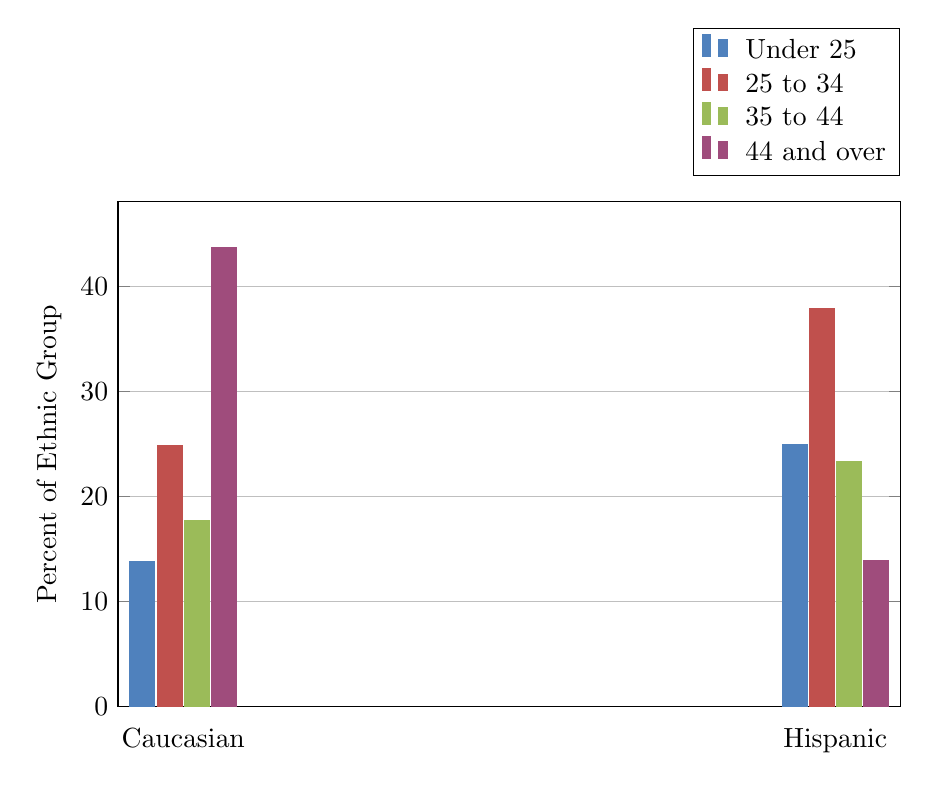
\begin{tikzpicture}
    \begin{axis}[
        width  = 0.95*\textwidth,
        height = 8cm,
        major x tick style = transparent,
        ybar=2*\pgflinewidth,
        bar width=9pt,
        ymajorgrids = true,
        ylabel = {Percent of Ethnic Group},
        symbolic x coords={Caucasian, Hispanic},
        xtick = data,
        scaled y ticks = false,
        ymin=0,
        legend cell align=left,
        legend style={
                at={(1,1.05)},
                anchor=south east,
                column sep=1ex
        }
    ]
        \addplot[style={bblue,fill=bblue,mark=none}]
            coordinates {(Caucasian, 13.8) (Hispanic, 24.9)};

        \addplot[style={rred,fill=rred,mark=none}]
             coordinates {(Caucasian, 24.8) (Hispanic, 37.9)};

        \addplot[style={ggreen,fill=ggreen,mark=none}]
             coordinates {(Caucasian, 17.7) (Hispanic, 23.3)};

        \addplot[style={ppurple,fill=ppurple,mark=none}]
             coordinates {(Caucasian, 43.7) (Hispanic, 13.9)};

        \legend{Under 25,25 to 34,35 to 44,44 and over}
    \end{axis}
\end{tikzpicture}
\item[]
\item[]
From the bar graph above, it is easy that
over 40\% of Caucasian visitors are older than 45.
Also, it should be noted that, on average, Hispanic visitors are younger.
\end{itemize}

\newpage

\item[25.5]
\begin{itemize}
\item[(a)]
Let's first build a table of expected counts.
\begin{center}
    \begin{tabular}{ |c|c|c|c| }
    \hline
     & Caucasian & Hispanic & Row Total\\
    \hline
    Under 25     & 209.3  & 50.7  & 260\\
    25 to 34     & 357.4  & 86.6  & 444\\
    35 to 44     & 246.3  & 59.7  & 306\\
    45 and over  & 495.0  & 120.0 & 615\\
    \hline
    Column Total & 1308.0 & 317.0 & 1625\\
    \hline
    \end{tabular}
\end{center}
\item[]
From the table above, it is easy to see
that row and column totals agree with the
totals for the observed counts.

\item[]

\item[(b)]
Hispanic visitors are, on average,
younger than Caucasian visitors
since the expected counts are smaller
than the observed counts for the Caucasians
in the older age categories.
Besides, observed counts are greater than
the expected counts for younger age
groups of Hispanics.
\end{itemize}

\item[]
\item[]

\item[25.7]
\begin{itemize}
\item[(a)]
The cell-count requirement is satisfied
as the expected counts are 209.28, 50.72, 357.39, 86.614,
246.31, 59.694, 495.03, 119.97 and all of these expected
counts are greater than 5.

\item[]

\item[(b)]
$\text{H}_0: \text{there is no relationship between ethnic group and age
of Monterey Bay Aquarium visitors}$.\\
$\text{H}_a: \text{there is a relationship between ethnic group and age
of Monterey Bay Aquarium visitors}$.\\
SAS output shows that $\chi^2 = 99.6058$ and $P < 0.0001$.

\item[]

\item[(c)]
The most significant difference is that Hispanic people visits
the aquarium at younger ages. Now, since every cell contributes
to $\chi^2$ and the more the difference between the expected and observed, the more the contribution, cells in the Hispanics column contribute the most.
\end{itemize}

\item[]
\item[]

\item[25.11]
\begin{itemize}
\item[(a)]
Since there was one sample which was then categorized by two variables,
we need to use the chi-square test of independence.

\item[]

\item[(b)]
We start with the \und{\textbf{PLAN}} part as the \und{\textbf{STATE}}
part is the description of the problem itself.\\\\
\und{\textbf{PLAN}}\\
Then our null hypothesis is $\text{H}_0: \text{there is no relationship between the age and how politically}$
informed a person is and the alternative
hypothesis is $\text{H}_\text{a}: \text{there is a relationship between the}$ age and how politically informed a person is.
\newpage
\und{\textbf{SOLVE}}\\\\
Since all expected counts are greater than 5, we can use the chi-procedures.
We have $\chi^2 \approx 32.062$ and $\text{df} = 12$ with $0.001 < \text{P} < 0.0025$ which.
\\\\\\
\und{\textbf{CONCLUDE}}\\
Since $0.001 < \text{P} < 0.0025 < 0.05$, we reject the null hypothesis
$\text{H}_0$ and conclude that there is a relationship between the age and how politically informed a person is.
\end{itemize}

\item[]
\item[]

\item[25.12]
\begin{itemize}
\item[(a)]
$\text{df} = (r - a) \times (c - 1) = (4 - 1) \times (2 - 1) = 3 \times 1 = 3.$

\item[]

\item[(b)]
With $\chi^2 = 99.6058$ and $\text{df} = 3$, we have $\text{P} < 0.0005$
which indicates that the result from SAS is more precise that the result
from Table D. Besides, the P-value from the SAS output gives us a bigger evidence against the null hypothesis than the P-value from the Table D.

\item[]

\item[(c)]
$\text{df} = (r - a) \times (c - 1) = (4 - 1) \times (4 - 1) = 3 \times 3 = 9.$
\end{itemize}

\item[]
\item[]

\item[25.14]
We start with the \und{\textbf{PLAN}} part as the \und{\textbf{STATE}}
part is the description of the problem itself.\\\\
\und{\textbf{PLAN}}\\
Then our null hypothesis is $\text{H}_0: \text{there is no relationship between the bird strikes and}$
tilting windows down so that they reflect earth rather than sky and the
hypothesis is $\text{H}_\text{a}: \text{there is a relationship}$ between the bird strikes and tilting windows down so that they reflect earth rather than sky.\\\\
\und{\textbf{SOLVE}}\\\\
We first need to construct a table. We get:
\begin{center}
    \begin{tabular}{ |c|c|c|c|c| }
    \hline
    & Vertical & 20-degree tilt & 40-degree tilt & Total\\
    \hline
    Strikes     & 31  & 14 & 8 & 53\\
    \hline
    \end{tabular}
\end{center}
\item[]
From the data above, we get that $\chi^2 \approx 16.11$ and $\text{df} = 3 - 1 = 2$ with $\text{P} < 0.0005$ (from Table D)\\\\\
\und{\textbf{CONCLUDE}}\\
Since $\text{P} < 0.0005 < 0.05$, we reject the null hypothesis
$\text{H}_0$ and conclude that there is a relationship between the bird strikes and tilting windows down so that they reflect earth rather than sky.

\item[]
\item[]

\item[25.15]
\begin{itemize}
\item[(a)]
If all days have the same probability, then $p_1 = p_2 = p_3 = p_4 = p_5 = p_6 = p_7 = \dfrac{1}{7}$ and we expect 100 births on every day.

\item[]

\item[(b)]
$\chi^2 = \dfrac{(84 - 100)^2}{100} + \dots + \dfrac{(72 - 100)^2}{100} = 19.12$.


\item[]

\item[(c)]
$\text{df} = c - 1 = 7 - 1 = 6$ with $0.0025 < \text{P} < 0.005 < 0.05$
which gives us a strong evidence that births are not spread evenly across
the week.
\end{itemize}

\end{itemize}
\end{document}
